\documentclass[main]{subfiles}

\begin{document}
\section{Databehandling}
\subsection{Modul et}

Som benævnt i \cref{dataopsamling1} er der indsamlet data med afstanden $d$ mellem nulte og første orden som funktion af $f_S$. Der er taget tre målinger af $d$ for den enkelte frekvens, som varieres fra $120$ til $280 \ \si{\mega\hertz}$ med spring af $10$ $\si{\mega\hertz}$ mellem hver måling. Grunden til de tre målinger pr. frekvens er for at komme tættere på en sand værdi med usikkerheder for hvert punkt, som her er valgt til at være standardafvigelsen på de tre målinger, altså således at $\text{sds}_{\text{std}} = \text{std}$. Målingspunkterne som ses på \cref{fig:rawdata_modul1} har centrum i gennemsnitsværdien af de tre målinger. Ydermere er tillagt en usikkerhed i målinger med lineal på
$ \text{sds}_{\text{lin}} = 1 \si{\milli\meter} $
. Altså er de endelige usikkerheder som ses på \cref{fig:rawdata_modul1}: $ \text{sds}_{\text{tot}} = \text{sds}_{\text{std}} + \text{sds}_{\text{lin}} $.
\begin{figure}[H]
    \centering
    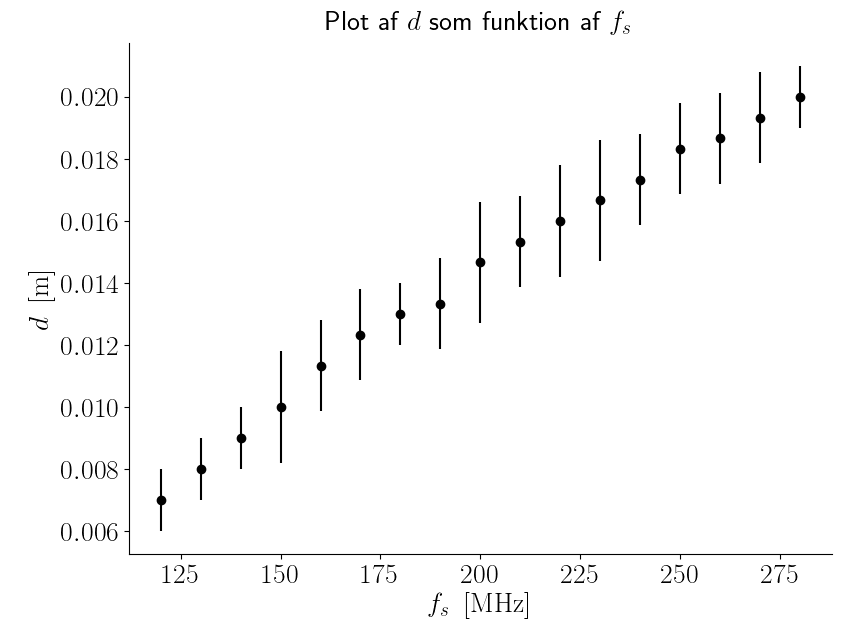
\includegraphics[width=\linewidth]{tegninger/rawdata_modul1.png}
    \caption{}
    \label{fig:rawdata_modul1}
\end{figure}
Idet at vi nu kender afstanden fra AOM'en ud til skærmen og afstanden mellem nulte og første orden, kan vi nu finde vinklen $\theta_{sep}$ ved \cref{eq:sep}.
Dette muliggører en afbildning af $\theta_{sep}$ som funktion af $f_S$. Denne fittes hvorved lydens hastighed kan bestemmes.
På figur \cref{fig:graf1} ses $\theta_{sep}$ plottet som funktion af $f_s$, med indlagt fit på data. Usikkerhederne på denne graf er bestemt ved ophobningsloven idet at usikkerhederne på $l$ og $d$ er kendte.
%TODO vurder om vi lige skal vise udregningen af usikkeden her
\begin{figure}[H]
    \centering
    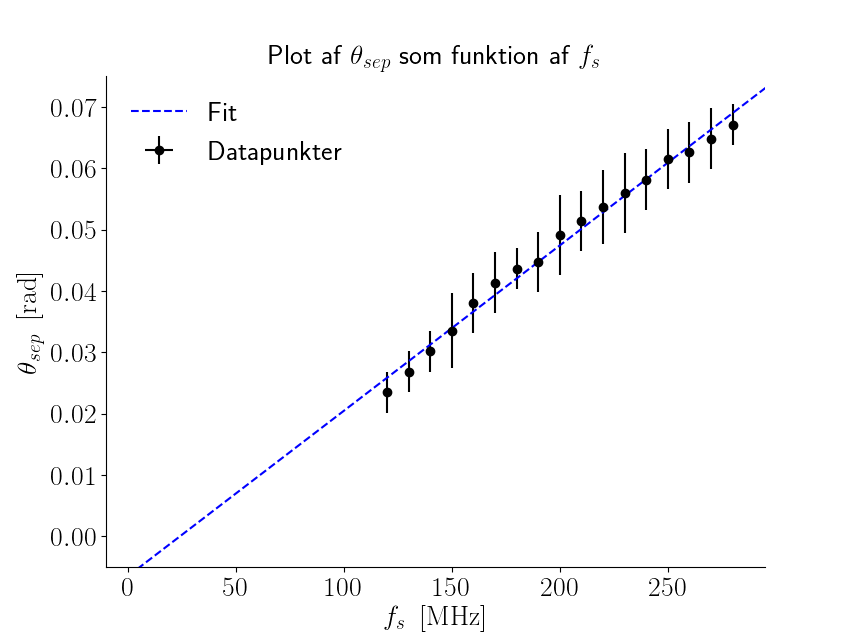
\includegraphics[width=\linewidth]{tegninger/graf1.png}
    \caption{}
    \label{fig:graf1}
\end{figure}
Det ses på \cref{fig:graf1} at den fittede kurve ikke skærer i $(0,0)$, hvilket den burde grundet udtrykket i \cref{eq:sep}.

Ydermere ses det at linjen skærer datapunkterne indenfor deres usikkerhedsfaner. Det ses fra \cref{eq:sep} at hældningen, $k_{\text{gradient}}$ på linjen bliver $ k_{\text{gradient}} = \frac{\lambda_L}{v_S}$, og da $k_{\text{gradient}} = \SI{0,213}{\second}$ kan finde lydens hastighed i krystallen til at være:
\begin{equation}
    \nonumber v_S = \frac{\lambda_L}{k_{\text{gradient}}} = 3377 \pm \ 89 \si{\meter\per\second}
\end{equation}
Usikkerheden på lydhastigheden er fundet ud fra spredningen på parametren $k_{\text{gradient}}$ ud fra fitte kommandoen \texttt{scipy.stats.linregress} som er en funktion fra python pakken \texttt{scipy}. Funktionen benytter mindste kvadraters metode. Ud fra spredningen på $k_{\text{gradient}}$ findes da usikkerheden på lydhastigheden, $v_S$ som:
\begin{equation}
    \nonumber sds(v_S) = \sqrt{\left(\frac{\lambda_L}{k_{\text{gradient}}^2}\right)^2 \cdot sds(k_{\text{gradient}})^2} = \SI{89}{\meter\per\second}
\end{equation}
Heri er det antaget at usikkerheden på bølgelængden af laseren er konstant, hvilket er grundet manglende informationer omkring laseren. Ydermere vil laseren sandsynligvis bidrage med en neglibel usikkerhed ift. \ usikkerheden som skyldes vores dataopsamling.

\bigskip

Der er taget målinger af intensiteten, $I_1$ af første ordens laserstrålen mens effekten til AOM'en varieres. Disse er afbildet på \cref{fig:graf2}. Usikkerhederne på denne måling kommer fra  powermeteret, der aldrig gav en konstant værdi, men tværtimod svinger om en punkt. %TODO blev vi ikke enige om at drengene fra 4.'s maskine ikke havde usikkerder?

\begin{figure}[H]
    \centering
    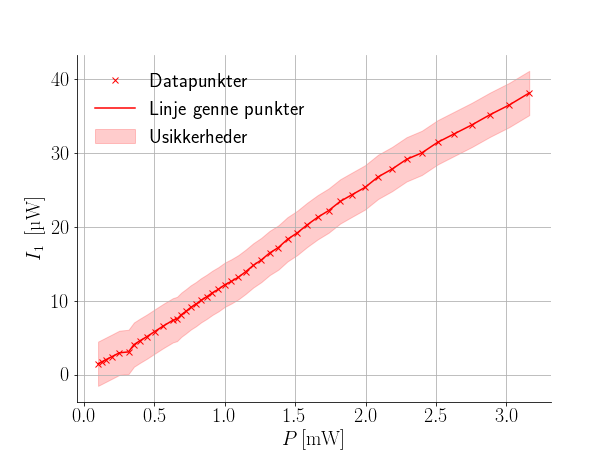
\includegraphics[width=\linewidth]{tegninger/graf2.png}
    \caption{}
    \label{fig:graf2}
\end{figure}
Egentlig skulle \cref{fig:graf2} være en figur som afbilder $\frac{I_1}{I_0}$ som funktion af effekten til AOM'en. Disse målinger skulle vise effektiviteten af diffraktionen, speciel skulle man se en mætning af effektiviteten. Man vil altså forvente en værdi for effekten til AOM'en som maksimerer effektiviteten af diffraktionen. Dette er dog ikke muligt at vise her idet at der mangles data til at udføre dette, navnligt mangles der målinger for $I_0$.



\end{document}
